\normalfalse\difficiletrue\tdifficilefalse
\correctionfalse

%\UPSTIidClasse{11} % 11 sup, 12 spé
%\newcommand{\UPSTIidClasse}{11}

\exer{Stabilisteur gyroscopique de bateau$\star$ \label{SLCI:03:96}}

% Concours Banque PT SIA -  2011

\setcounter{question}{0}\marginnote{\xpComp{SLCI}{03}}%\UPSTIcompetence{B2-07}
\index{Compétence B2-07}\index{Compétence SLCI-03}
\index{Schéma-blocs}
\index{Stabilisateur}
\ifcorrection
\else
\marginnote{\textbf{Pas de corrigé pour cet exercice.}}
\fi

\ifprof
\else
%\section*{Présentation du système}
Soit le schéma-bloc suivant de la figure \ref{SLCI:03:96:fig:01}.

\begin{figure}[!h]
\centering
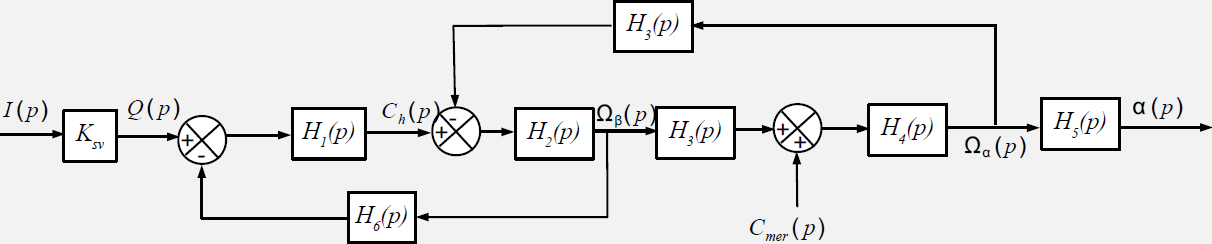
\includegraphics[width=\linewidth]{96_01}
\caption{\label{SLCI:03:96:fig:01} Modélisation de la commande du vérin}
\end{figure}

\begin{marginfigure}
\centering
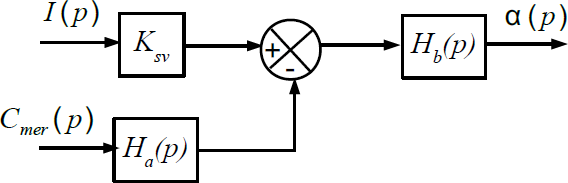
\includegraphics[width=\linewidth]{96_02}
\caption{\label{SLCI:03:96:fig:02} Modèle simplifié}
\end{marginfigure}

\question{Montrer que le schéma-bloc de la figure \ref{SLCI:03:96:fig:01} peut se mettre sous la forme du schéma de la figure \ref{SLCI:03:96:fig:02}.}

\ifprof
\else
\marginnote{Corrigé voir \ref{SLCI:03:96}.}
\fi